\documentclass[letter,10pt]{article}
\usepackage[utf8x]{inputenc}
\usepackage{graphicx}

%opening
\title{Agile Integer Linear Programming Solutions for Floating Sensors}
\author{Kevin Weekly}

\begin{document}

\maketitle

\begin{abstract}
This project will focus on identifying and solving problems related to coordination and control of motorized floating sensor units. We predict there are a range of problems related to task assignment and maneuver selection which are valuable to a continuously operating fleet of sensors.  We also predict that applying integer programming or combinatorial algorithms to obtain optimal solutions will be a marked improvement over greedy, heuristic, or human-chosen approaches.

The intent is that such problems can be solved repeatedly during a deployment as conditions about the environment are discovered, or the user requirements change.  Therefore, the problems should be able to be solved on a modern desktop computer using either CPLEX or corresponding Python libraries (preferred) in the order of minutes or less.  Also, there may also be some benefit in examining the Lagrange multipliers from these problems to furnish the user with information on the way that constraints are affecting the solution. 
\end{abstract}

\section{The Floating Sensor Network}

The floating sensor network is a fleet of 20 motorized sensors, or ``drifters'', used currently to measure the Lagrangian flow-field of their environment.  A graphical depiction of one sensor is shown in Figure \ref{fig:fsn-drifter}. 

During a deployment operation, the fleet of 20 are deployed in a region of the San-Joaquin/Sacramento Delta where they float along with the natural current, reporting their GPS position \& salinity measurements over the GSM (cell-phone) network or Zigbee (short-range radio) network.  In the context of deployment, there are effectively two sets of variables we could optimize over--
\begin{itemize}
 \item The individual deployment strategy for the fleet from a boat. i.e. when, where, and how many units are deployed from a human-operated motorboat.  This strategy is constrained by the limited speed of boats, their limited mobility in shallow areas (i.e. the drifters can go to some places the boats cannot), and limited capacity (typically can carry 5 units).
 \item The actuation of the drifters themselves.  Using their motors, the units can move themselves in any direction, albiet slowly.  Their control authority is approximately $20 \frac{\mbox{cm}}{\mbox{s}}$ \emph{relative to the water speed} (i.e. in some areas the current is fast enough that the units cannot swim upstream).  They are further constrained by limited battery life, and, were the proposed algorithm to be done in a centralized manner, by lack of communication.
\end{itemize}


\begin{figure}[h]
 \centering
 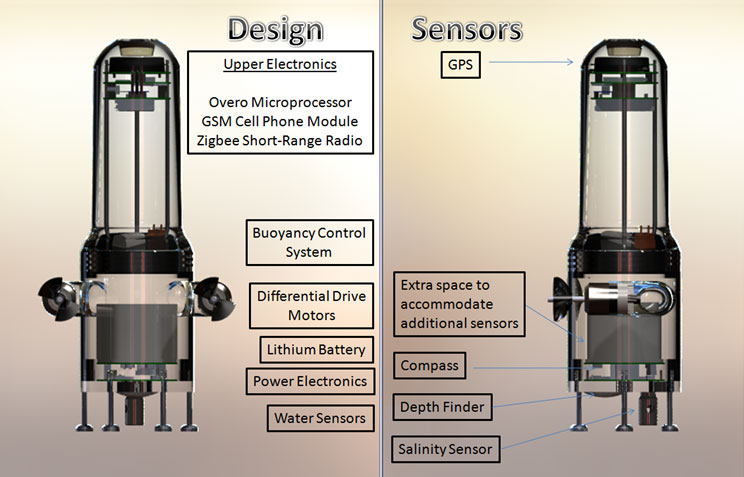
\includegraphics[width=\linewidth ]{figures/fsn.jpg}
 \caption{Floating Sensor Unit\label{fig:fsn-drifter}}
\end{figure}


\end{document}
